

\documentclass[
	11pt,
]{beamer}

\graphicspath{{Images/}{./}}

\usepackage{booktabs}
\usepackage[backend=bibtex, style=authoryear, bibstyle=authoryear, citestyle=authoryear, natbib=true, sorting=none]{biblatex}
\usepackage[backend=bibtex, style=authoryear, bibstyle=authoryear, citestyle=authoryear, natbib=true, sorting=none]{biblatex}
\usepackage{array}
\newcolumntype{M}[1]{>{\centering\arraybackslash}m{#1}}

\setlength{\arrayrulewidth}{0.5mm}
\setlength{\tabcolsep}{6pt}
\renewcommand{\arraystretch}{1.2}

\bibliography{references.bib}



\usetheme{CambridgeUS}



\usecolortheme{seahorse}
                


\usefonttheme{default}


\usepackage{palatino}

\usepackage[default]{opensans}



\useinnertheme{circles}







\title[Deep Learning with Data Maps]{Evaluating and Crafting Datasets Effective for Deep Learning With Data Maps}


\author[Institute for Computing in Research]{Jay Bishnu \and Andrew Gondoputro}

\institute[ICR]{Institute for Computing In Research \\ \smallskip }

\date{\today}


\begin{document}


\begin{frame}
	\titlepage
\end{frame}



\begin{frame}
	\frametitle{Guiding Questions}
	\fontsize{18}{20}\selectfont
	\begin{block}
		\huge How can we assess the quality of a dataset?
	\end{block}
	\vspace{0.5in}
	\begin{block}
		\huge What types of samples are best for building high-quality datasets?
	\end{block}
\end{frame}


\section{Background}


\subsection{Natural Language Processing}
\begin{frame}
	\frametitle{Natural Language Processing}
	\framesubtitle{}

	\begin{itemize}
		\item Natural language processing (NLP)
		      \begin{itemize}
			      \item Text categorization
			      \item Text filtering
			      \item Sentiment analysis
		      \end{itemize}
		\item Example: given the text of a movie review, a model predicts the rating (in stars) for that review
	\end{itemize}

	\bigskip

\end{frame}

\subsection{Training}
\begin{frame}{Training}
	\begin{itemize}
		\item Supervised learning: samples in a dataset are labeled by humans
		      \begin{itemize}
			      \item For deep learning, data sets are generally at least 10,000 samples long
			      \item Larger data sets are often better for training, but take longer to process (\cite{banko-brill-2001-mitigating})
		      \end{itemize}
		\item Datasets are often divided into three "splits"
		      \begin{itemize}
			      \item Train split: the samples on which the model is trained (in-distribution)
			      \item Dev split: the samples on which the model is evaluated to make sure it is learning during training
			      \item Test split: the samples on which the model is tested to produce a final accuracy measurement
		      \end{itemize}
	\end{itemize}
\end{frame}


\subsection{The SNLI Dataset}
\begin{frame}{The SNLI Dataset}
	\framesubtitle{Stanford Natural Language Inference}
	\begin{itemize}
		\item Dataset with more than 500,000 samples (\cite{snli:emnlp2015})
		\item Sentences are paired and labeled
		      \begin{itemize}
			      \item Entailment: if Sentence 1 is true, Sentence 2 must also be true
			      \item Contradiction: if Sentence 1 is true, Sentence 2 cannot be true
			      \item Ambiguous: If Sentence 1 is true, Sentence 2 could be either true or false
		      \end{itemize}
	\end{itemize}
	\vspace{.2cm}
	\fontsize{8pt}{10pt}\selectfont
	\begin{tabular}{| M{4.1cm} | M{4.1cm}| M{2cm} |}
		\hline
		Sentence 1                                                                & Sentence 2                                       & Gold Label    \\ \hline
		Three black dogs on grass.                                                & Three dogs on grass.                             & Entailment    \\ \hline
		Three men are sitting on chairs.                                          & The men are dancing together on the dance floor. & Contradiction \\ \hline
		Short dark hair woman with a black phone is on the phone on the sidewalk. & A woman is on the phone with her husband.        & Neutral       \\
		\hline
	\end{tabular}
\end{frame}



\section{Dataset Cartography}

\subsection{Data Maps}
\begin{frame}[t]{Data Maps}
	Data maps - visual representation of sample performance from training
	(\cite{swayamdipta2020dataset})
	\vspace{0.5cm}
	\begin{columns}[t]
		\begin{column}{.5\textwidth}
			Metrics
			\begin{itemize}
				\item Confidence
				      \begin{itemize}
					      \item On average, how confident is the model in predicting the correct label?
				      \end{itemize}
				\item Variability
				      \begin{itemize}
					      \item How much does confidence vary across epochs?
				      \end{itemize}

			\end{itemize}
		\end{column}
		\begin{column}{.5\textwidth}
			Categorization of Data
			\begin{itemize}
				\item Easy-to-learn
				      \begin{itemize}
					      \item High confidence and
					            low variability
				      \end{itemize}
				\item Hard-to-learn
				      \begin{itemize}
					      \item Low confidence and low varability
				      \end{itemize}
				\item Ambiguous
				      \begin{itemize}
					      \item High variability
				      \end{itemize}
			\end{itemize}
		\end{column}
	\end{columns}
\end{frame}

\subsection{Cloud Computing Solution}
\begin{frame}{Cloud Computing Solution}
	\framesubtitle{Google Cloud Platform}
	\begin{columns}
		\begin{column}{.4\textwidth}

			
\includegraphics[scale=0.6]{gcp.png}
		\end{column}
		\begin{column}{.6\textwidth}
			\begin{itemize}
				\item Nvidia Tesla V100 GPU
				\item 4 vCPU w/ 15 GiB memory
				\item Can run for long periods without interruption
			\end{itemize}
		\end{column}
	\end{columns}
\end{frame}

\subsection{Data Map Example}
\begin{frame}[t]{Data Map Example}
	\centering
	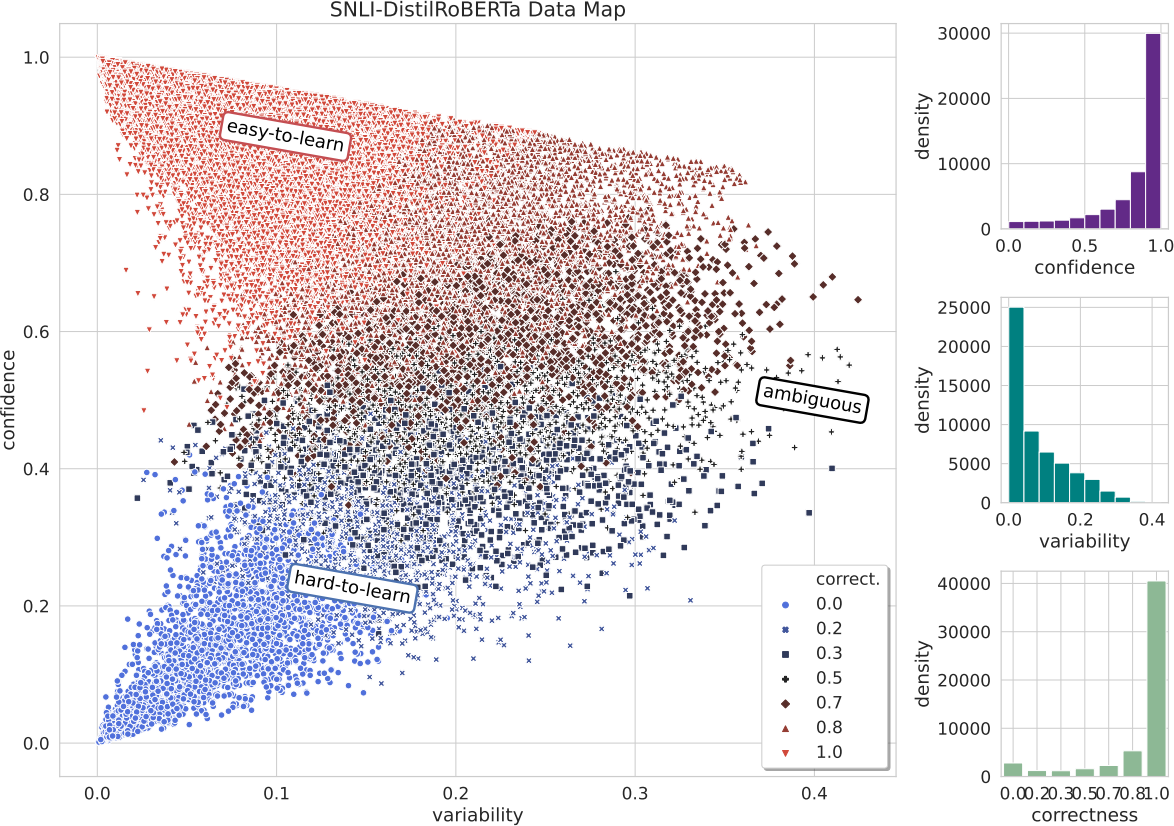
\includegraphics{data_map.png}
\end{frame}

\section{Experiment}

\subsection{Our Experiment}
\begin{frame}[t]{Our Experiment}
	\begin{block}{Goal}
		Minimize the size of a training dataset while maximizing accuracy using the dataset cartography
	\end{block}
	\begin{columns}[t]
		\begin{column}{.5\textwidth}
			\begin{itemize}
				\item Test models trained on each of the categories of data
				\item Find what mixes of subsets work best
			\end{itemize}
		\end{column}
		\begin{column}{.5\textwidth}
			\begin{itemize}
				\item Compare different results for the most "efficient" training dataset
			\end{itemize}
		\end{column}
	\end{columns}
\end{frame}


\subsection{Controls and Benchmarks}
\begin{frame}[t]{Controls and Benchmarks    }
	\begin{columns}[t]
		\begin{column}{.5\textwidth}
			Controls
			\begin{itemize}
				\item Datasets are randomized right before training to remove any order bias
				\item Same number of data instances in everything but the baseline
				\item 6 Epoch training
				\item Same accuracy datasets for tests
				\item Use the \% most of each category
			\end{itemize}
		\end{column}
		\begin{column}{.5\textwidth}
			Benchmarks
			\begin{itemize}
				\item 100\% of the dataset randomized
				\item 33\% of the dataset randomized
			\end{itemize}
		\end{column}
	\end{columns}
\end{frame}

\subsection{Data Subsets}
\begin{frame}{Data Subsets}
	\begin{columns}
		\begin{column}{.4\textwidth}
			\begin{itemize}
				\item 100\% Random
				\item  33\% Random
				      \vspace{1cm}
				\item 33\% Easy-to-learn
				\item 33\% Hard-to-learn
				\item 33\% Ambiguous
			\end{itemize}
		\end{column}
		\begin{column}{.6\textwidth}
			\begin{itemize}
				\fontsize{11pt}{20pt}\selectfont
				\item 16\% easy, 16\% hard
				\item 16\% easy, 16\% ambiguous
				\item 16\% hard, 16\% ambiguous
				\item 11\% easy, 11\% hard, 11\% ambiguous
			\end{itemize}

		\end{column}
	\end{columns}
\end{frame}


\subsection{Methods}
\begin{frame}[t]{Methods}
	\vspace{.5cm}
	\begin{enumerate}
		\fontsize{11pt}{20pt}\selectfont
		\item Run training normally on 6 epochs, categorizing data
		\item Filter training data to create appropriate subsets
		\item Shuffle all sets to avoid order bias
		\item Train a new model with each data subset
		\item Evaluate performance with the out-of-distribution sets
	\end{enumerate}
\end{frame}



\section{Results}

\subsection{Final Accuracies}
\begin{frame}
	\frametitle{Final Accuracies}
	\begin{table}
		\fontsize{8pt}{10pt}\selectfont
		\centering
		\begin{tabular}{| m{4cm} | M{2cm} | M{2cm} | M{2cm} |}
			\hline
			~                                                                           & Final Training Accuracy (ID) & Dev \newline Accuracy (OOD) & Test \newline Accuracy (OOD) \\ \hline
			100.00\% random                                                             & 0.8936                       & 0.8997                      & 0.8976                       \\ \hline
			33.33\% random                                                              & 0.8782                       & 0.8776                      & 0.8785                       \\ \hline
			33.33\% easy-to-learn                                                       & 0.9996                       & 0.8293                      & 0.8286                       \\ \hline
			33.33\% hard-to-learn                                                       & 0.5680                       & 0.5966                      & 0.5856                       \\ \hline
			33.33\% ambiguous                                                           & 0.7684                       & 0.8878                      & 0.8894                       \\ \hline
			16.67\% easy-to-learn\newline16.67\% hard-to-learn                          & 0.7581                       & 0.5938                      & 0.5999                       \\ \hline
			16.67\% easy-to-learn\newline16.67\% ambiguous                              & 0.8835                       & 0.8802                      & 0.8807                       \\ \hline
			16.67\% hard-to-learn\newline16.67\% ambiguous                              & 0.5900                       & 0.4076                      & 0.4023                       \\ \hline
			11.11\% easy-to-learn\newline11.11\% hard-to-learn\newline11.11\% ambiguous & 0.7401                       & 0.5249                      & 0.5145                       \\ \hline
		\end{tabular}
	\end{table}
\end{frame}

\subsection{Mislabeled Data}
\begin{frame}{Mislabeled Data}
	\framesubtitle{Hard-to-learn examples}
	\begin{table}
		\fontsize{8pt}{10pt}\selectfont
		\centering
		\begin{tabular}{| M{3cm} | M{3cm} | M{2cm} | M{2cm} |}
			\hline
			Sentence 1                                                             & Sentence 2                                        & Gold Label    & Our Label     \\ \hline
			A hiker travels along a rocky path bordered by greenery.               & The hiker is carrying a big backpack on his back. & Entailment    & Neutral       \\ \hline
			Two beige dogs are playing in the snow.                                & Two dogs are outside.                             & Contradiction & Entailment    \\ \hline
			A man with a gray beard is standing next to a woman in a brown jacket. & Nobody is standing.                               & Neutral       & Contradiction \\
			\hline
		\end{tabular}
	\end{table}
\end{frame}



\section{Further Research}

\subsection{Next Steps}
\begin{frame}{Next Steps}
	\fontsize{12pt}{16pt}\selectfont
	\begin{itemize}
		\item Other datasets
		      \vspace{.5cm}
		\item Applications to other models (generative adversarial networks)
		      \vspace{.5cm}
		\item Managing mislabeled samples
	\end{itemize}
\end{frame}

\section{Bibliography}

\subsection{References}
\begin{frame}{References}
	\nocite{*}
	\printbibliography
\end{frame}



\begin{frame}[plain]
	\begin{center}


		{\LARGE Questions?}
	\end{center}
\end{frame}


\end{document}